\documentclass[conference]{IEEEtran}
\IEEEoverridecommandlockouts
\usepackage{cite}
\usepackage{amsmath,amssymb}
\usepackage{graphicx}
\usepackage{booktabs}
\usepackage{xcolor}
\usepackage{url}
\graphicspath{{figs/}}

\begin{document}

\title{Cause-Aware Tabular Q-Learning for NB-IoT Random Access over LEO Satellites: An Energy--Latency Study on Real Orbital Passes}

% TODO(author): add co-authors / guide, department, institution, city, country, e-mail.
\author{\IEEEauthorblockN{Purvil Patel}
\IEEEauthorblockA{\textit{Department (to be completed)}\\
\textit{Institution (to be completed)}}}

\maketitle

\begin{abstract}
Narrowband IoT (NB-IoT) over low-Earth-orbit (LEO) satellites can serve smart meters outside terrestrial coverage. However, its random-access (RA) parameters were designed for static terrestrial cells. We study a lightweight tabular Q-learning controller that jointly sets the access-barring factor, the Backoff Indicator and the NPRACH repetition profile at every RA opportunity. It uses only quantities a base station can observe: idle, detected and collided subcarriers, Msg3 failures, and ephemeris-derived elevation. From these, a maximum-likelihood estimator recovers the load and the dominant failure cause (collision, detection miss, or timeout of meters with a stale GNSS fix). We evaluate the controller on 14 real SGP4 passes of an operational NB-IoT nanosatellite, with a TR~38.821 Set-4 link budget and a detection model anchored to TS~36.104. The comparison includes static, heuristic, terrestrial-trained and exhaustive-search baselines, with 10 traffic seeds per pass and paired significance tests. At nominal load, the controller matches a static NTN-aware configuration in 10-s access success (0.668 vs.\ 0.663) with 9\% less preamble airtime, and none of the 60 fixed configurations is better on both metrics. It remains 6--8 percentage points (pp) below a channel-aware heuristic and the best fixed configuration, which spend ${\sim}60\%$ more airtime. When the load is 3--5$\times$ the nominal value, it outperforms the best fixed configuration by 4.6--8.1~pp. Cause information adds 1.4--1.6~pp, whereas satellite geometry in the state gives no measurable gain. We report this negative result together with one pre-declared design iteration.
\end{abstract}

\begin{IEEEkeywords}
NB-IoT, non-terrestrial networks, LEO satellite, random access, access barring, Q-learning.
\end{IEEEkeywords}

\section{Introduction}
Release~17 brought NB-IoT into non-terrestrial networks (NTN), so a satellite can act as the base station for meters that no terrestrial cell reaches. The NB-IoT random-access channel (NPRACH) changes character over such a link. One-way delay varies between 2 and 6.3~ms during a pass. The uplink signal-to-noise ratio (SNR) of a nanosatellite payload swings by about 15~dB between horizon and zenith~\cite{dwivedi2024efficient}. Visibility is bounded to a few minutes~\cite{dwivedi2024efficient,le2024survey}. Access-control parameters (barring, backoff and repetitions) are still configured as in terrestrial cells.

Three bodies of work touch this problem, but do not meet. First, learning-based access-class barring (ACB) and NPRACH tuning works well terrestrially~\cite{tello2018acb,bui2020drlacb,abera2025ddqn,jiang2019rl,daraseliya2026reactive}, but assumes a static channel. Second, NB-IoT NTN studies model delay, Doppler and detection carefully~\cite{chougrani2022nbiot,lin2025unified,kodheli2021ra,shen2025leo}, but leave access control at its defaults. Third, learning for LEO random access targets other knobs, such as RAO allocation~\cite{liu2022dyna}, backoff and association~\cite{lee2023erach}, channel selection~\cite{feng2026joint} or SCMA codebooks~\cite{wu2025scma}. The closest works optimise multi-class ACB and the RACH period analytically~\cite{chen2026channel}. Others detect preamble collisions at the satellite~\cite{jeong2025mtecd,jeong2026isc,lee2025dl}. Lee \emph{et al.}~\cite{lee2025dl} explicitly name combining collision-type estimation with reinforcement learning as an open direction.

This paper takes that step and evaluates it against strong references. Our contributions are:
\begin{itemize}
\item An \emph{observable} controller formulation. A grid maximum-likelihood estimator turns per-subcarrier NPRACH observations into load, collision, miss and timeout estimates. These feed a 108-state, 60-action Q-table (52~KB) that jointly sets barring, backoff and the per-CE-level repetition profile.
\item A simulation grounded in real geometry and standards. It uses SGP4 passes of an operational satellite, a TR~38.821 Set-4 link budget, a detection curve through the TS~36.104 NPRACH requirements, and per-meter coverage-enhancement (CE) levels. Timeouts come from meters with a stale GNSS fix.
\item An honest evaluation. The proposed controller is compared with static, heuristic, terrestrial-trained and exhaustive-search (genie) baselines, plus two ablations. We use 140 paired runs per scheme, sensitivity sweeps, and full disclosure of one pre-declared design iteration.
\end{itemize}

\section{System Model}
\subsection{Orbit and Geometry}
We propagate four real Sateliot TLEs (${\sim}577$~km, $97.7^\circ$ inclination, epoch Oct.~2026) with SGP4 for seven days, for a ground site in Ahmedabad, India. All 14 passes of the test satellite above a $10^\circ$ mask with a peak $\ge 20^\circ$ form the test set. Their peaks range from $20^\circ$ to $86^\circ$ and their durations from 364 to 490~s (Fig.~\ref{fig:geom}). Forty passes of the three other satellites are used only for pre-training. The one-way delay is 1.94--6.30~ms and the raw Doppler reaches $\pm 46$~kHz at 2~GHz, consistent with~\cite{chougrani2022nbiot,shen2025leo}.

\begin{figure*}[t]
\centering
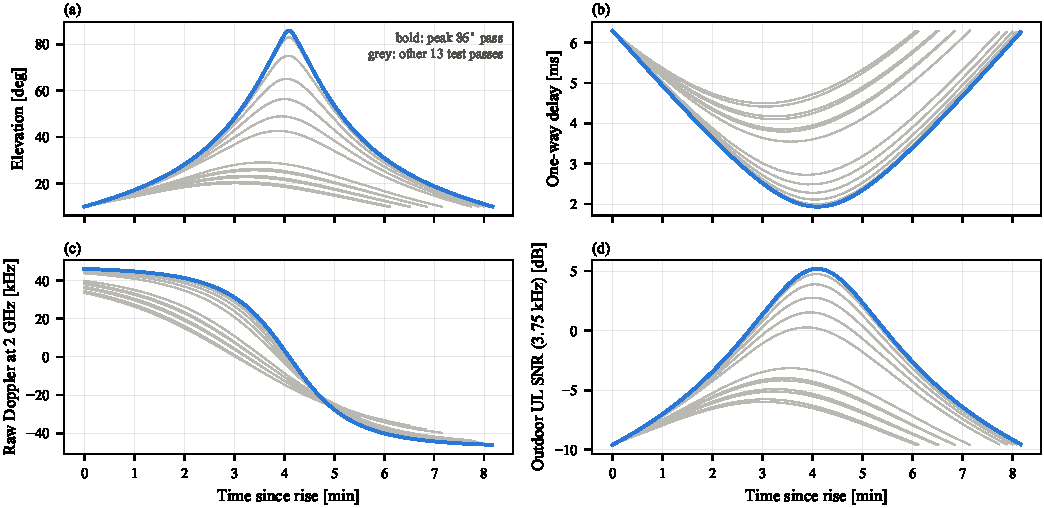
\includegraphics[width=\textwidth]{fig1_geometry.pdf}
\caption{Geometry of the 14 test passes (SGP4, real TLEs): (a) elevation, (b) one-way delay, (c) raw Doppler at 2~GHz, (d) outdoor uplink SNR in 3.75~kHz from the Set-4 link budget. The highest pass is highlighted.}
\label{fig:geom}
\end{figure*}

\subsection{Link Budget and Detection}
The single-tone uplink SNR follows the Set-4 budget of~\cite{dwivedi2024efficient}, based on~\cite{3gpp38821}. It uses a UE EIRP of $-7$~dBW and a satellite $G/T$ of $-18.6$~dB/K. The atmospheric, shadowing, scintillation and polarisation losses are 0.1, 3, 2.2 and 3~dB. The beam roll-off is $12(\theta/104.7^\circ)^2$~dB at off-nadir angle $\theta$, and the bandwidth is $B=3.75$~kHz. It reproduces the published $-3.14$~dB at $30^\circ$ and $+4.93$~dB at $90^\circ$. Each meter adds a fixed coupling loss $L_i\sim\mathcal N(\mu_L,4\,\mathrm{dB})$, which represents installation and building penetration; $\mu_L$ is our stress axis. The detection probability of a preamble with $N$ repetitions is
\begin{equation}
P_d=\big[1+e^{-k(\mathrm{SNR}-\mathrm{SNR}_{99}(N))-\ln 99}\big]^{-1},
\end{equation}
where $\mathrm{SNR}_{99}(N)=0.9-2.35\log_2(N/8)+\Delta$~dB and $k=1.2$~dB$^{-1}$. This curve passes exactly through the TS~36.104 AWGN requirements~\cite{3gpp36104} ($99\%$ at $-2.1$~dB for 8 repetitions and $-6.8$~dB for 32, with 2 receive antennas), shifted by $+3$~dB for a single receive branch. We use $\Delta=0$ (GNSS-assisted, as in Rel-17). A GNSS-free regime uses $\Delta=10.3$~dB, a least-squares fit ($\pm1.4$~dB) to Chougrani \emph{et al.}~\cite{chougrani2022nbiot}. Residual Doppler after pre-compensation (${\sim}10$~Hz~\cite{r12100601}, up to 250~Hz~\cite{lee2025dl}) is below 7\% of the 3.75-kHz subcarrier spacing and costs $<0.1$~dB, so we do not model it.

\subsection{Random-Access Procedure and Failure Causes}
Decisions are taken every 320~ms. The model has three CE levels with 24, 12 and 12 NPRACH subcarriers and preamble format~1 (6.4~ms per repetition)~\cite{3gpp36211}. Each CE level has its own periodicity $m_k\cdot 320$~ms, long enough to fit its repetitions.

At RA initiation, a meter passes the NB-IoT access-barring bitmap, which we model as a pass probability $p$ over ten access classes. A barred meter waits $(0.7+0.6U)\cdot 4$~s. A meter that passes selects its CE level by comparing its measured SNR with the thresholds $\mathrm{SNR}_{99}(N_k)$.

Meters then pick subcarriers uniformly at random. Each attempt ends in exactly one ground-truth outcome:
\begin{itemize}
\item \emph{collision}: two or more meters on one subcarrier, with no capture;
\item \emph{miss}: a lone preamble that is not detected;
\item \emph{timeout}: a detected lone preamble from a meter with a stale GNSS fix ($10\%$ of meters) whose residual timing error $\sim U(0,\,2D\cos\epsilon/c)$, with $D=250$~km~\cite{chougrani2022nbiot}, exceeds the 266.7-$\mu$s cyclic prefix, so its Msg3 is lost;
\item \emph{success}.
\end{itemize}
After a timeout, the meter re-acquires GNSS with probability 0.5. A failed meter backs off $U(0,\mathrm{BI})$. It moves up one CE level after four failures and is dropped after ten~\cite{3gpp36321,3gpp36331}. Per pass, $N$ meters need access: 70\% periodic reports spread uniformly over the pass, plus a 30\% Beta(3,4) alarm burst over 10~s at a random time~\cite{3gpp37868}.

\section{Cause-Aware Q-Learning Controller}
\subsection{Observations and Estimator}
Per CE pool, the gNB observes four counts: successes; collided subcarriers flagged by an early collision detector with $P_{cd}=0.95$~\cite{jeong2025mtecd,jeong2026isc}; Msg3 failures; and idle-looking subcarriers. Under a slotted-ALOHA model with attempt rate $\lambda$ per subcarrier and mean detection probability $\bar P_d$, a subcarrier is collided with probability $1-e^{-\lambda}(1+\lambda)$, holds a detected singleton with probability $\lambda e^{-\lambda}\bar P_d$, and looks idle otherwise. A grid maximum-likelihood fit of $(\lambda,\bar P_d)$ to exponentially smoothed counts gives an estimate $\hat\lambda$. From it we obtain:
\begin{itemize}
\item attempts $\hat n=R\hat\lambda$, for a pool of $R$ subcarriers;
\item colliding meters $\hat c=R\hat\lambda(1-e^{-\hat\lambda})$;
\item misses $\hat m=\max(0,R\hat\lambda e^{-\hat\lambda}-s)$, where $s$ is the number of detected singletons;
\item timeouts $\hat t$, the Msg3 failures not explained by unflagged collisions.
\end{itemize}
In Monte-Carlo checks, the load bias is below 15\% and the miss error below one meter per opportunity.

\subsection{State, Action and Reward}
The state has four discretised components: load $\hat\lambda$ (3 bins), elevation (3 bins), pass phase (3 bins), and the dominant failure cause (4 bins: low, collision, miss, timeout), for 108 states in total. The action is the tuple (barring factor $p\in\{0.1,0.3,0.5,0.7,1\}$, BI $\in\{256,1024,4096,16384\}$~ms, repetition profile). The three repetition profiles set (CE0, CE1, CE2) to $\{2,8,32\}$, $\{4,16,64\}$ or $\{8,32,128\}$, giving 60 actions in total. The reward per decision epoch is
\begin{equation}
\begin{aligned}
r={}&\frac{w_s n_s-w_c\hat c-w_m\hat m-w_t\hat t}{R_{\mathrm{act}}}-w_e\frac{\sum_k \hat n_k N_k}{R_{\mathrm{act}}N_{\max}}\\
&-w_d\min\!\Big(\frac{\bar T_b\frac{1-p}{p}+\hat f\,\frac{\mathrm{BI}}{2}}{D},\,3\Big),
\end{aligned}
\end{equation}
with $(w_s,w_c,w_m,w_t,w_e,w_d)=(1,1,0.5,0.5,0.1,0.5)$. Here $R_{\mathrm{act}}$ is the number of active subcarriers, $\bar T_b=4$~s, $D=10$~s, and $\hat f$ is the estimated failure share. The last term is the expected wait that the chosen barring and backoff impose on a meter. The gNB knows every quantity in $r$, and a unit test verifies that ground-truth fields do not affect it.

\subsection{Learning}
We use Q-learning with $\alpha=0.12$ and $\gamma=0.9$. A \emph{warm-start} table is pre-trained on 120 passes of the training satellites with randomised $N$, $\mu_L$ and GNSS-degraded share, with $\varepsilon$ decaying from 1 to 0.05. It is then fine-tuned online ($\varepsilon=0.1$) during each test pass. A \emph{cold-start} variant learns from zero within the pass. We define two ablations: one keeps the cause state but replaces $(w_c,w_m,w_t)$ by their mean (lumped reward); the other also removes the cause bin from the state.

\section{Evaluation Setup}
We compare the following baselines:
\begin{itemize}
\item \textbf{B1}: fixed terrestrial-style configuration ($p=1$, BI~$=256$~ms, low repetition profile).
\item \textbf{B2}: static NTN-aware configuration ($p=0.7$, 1024~ms, mid profile). 3GPP defines no such default; we choose B2 as a moderate setting.
\item \textbf{B3}: the same learner trained on a \emph{terrestrial} channel (fixed 4.93-dB SNR, no delay, no GNSS errors), using only the load and cause state, and deployed frozen.
\item \textbf{B4}: a channel-aware heuristic that sets the repetition profile from elevation and the barring factor and backoff from $\hat\lambda$.
\item \textbf{B5}: the best of all 60 fixed actions found by exhaustive search on the test passes. B5 is a genie reference, not a deployable scheme.
\end{itemize}
All schemes see identical traffic, losses and GNSS flags for each (pass, seed), so comparisons are paired. The main metric is the fraction of meters served within $D=10$~s, $P_s^{\le D}$. We also report the served fraction within the pass, the drop rate, the delay, and the preamble airtime per served meter (an energy proxy). We report means with 95\% confidence intervals over 140 runs (14 passes $\times$ 10 seeds) and two-sided Wilcoxon signed-rank tests with Holm correction.

\begin{table}[t]
\caption{Main results, $N=1000$, $\mu_L=0$~dB (mean $\pm$ 95\% CI, 140 paired runs)}
\label{tab:main}
\centering
\setlength{\tabcolsep}{3pt}
\footnotesize
\begin{tabular}{lccccc}
\toprule
Scheme & $P_s^{\le D}$ & $P_s$ & Drop & $\bar d$ [s] & Airtime [ms]\\
\midrule
Proposed (warm) & $0.668{\pm}0.019$ & 0.756 & 0.223 & $4.06$ & $2034{\pm}164$\\
Proposed (cold) & $0.607{\pm}0.022$ & 0.794 & 0.164 & $7.37$ & $1803{\pm}143$\\
Abl.: lumped reward & $0.652{\pm}0.021$ & 0.737 & 0.231 & $3.97$ & $2040{\pm}149$\\
Abl.: no cause info & $0.654{\pm}0.019$ & 0.745 & 0.229 & $4.20$ & $2254{\pm}174$\\
B1 Fixed terrestrial & $0.619{\pm}0.016$ & 0.619 & 0.377 & $0.85$ & $1687{\pm}93$\\
B2 Static NTN-aware & $0.663{\pm}0.018$ & 0.722 & 0.262 & $3.49$ & $2246{\pm}147$\\
B3 Terrestrial-trained Q & $0.681{\pm}0.021$ & 0.755 & 0.217 & $3.84$ & $1912{\pm}140$\\
B4 Heuristic & $0.730{\pm}0.018$ & 0.773 & 0.204 & $2.71$ & $3259{\pm}268$\\
B5 Best fixed (genie) & $0.745{\pm}0.017$ & 0.775 & 0.208 & $2.14$ & $3367{\pm}236$\\
\bottomrule
\end{tabular}
\end{table}

\section{Results}
\subsection{Nominal Load}
Table~\ref{tab:main} gives the main comparison. All differences from the proposed controller in $P_s^{\le D}$ are significant ($p_{\mathrm{Holm}}<10^{-3}$).
\begin{itemize}
\item \emph{Against B2}, the controller achieves the same 10-s success ($+0.5$~pp), 3.9~pp fewer drops and 9\% less airtime. On the two exhaustive-search seeds, none of the 60 fixed actions is better than the proposed controller on both $P_s^{\le D}$ and airtime, whereas one fixed action ($p=1$, BI~$=4096$~ms, mid profile) dominates B2.
\item \emph{Against B4 and B5}, it trails by 6.1 and 7.7~pp. Both buy that margin with ${\sim}60\%$ more airtime: B5 runs the high-repetition profile throughout the pass, and B4 runs it at low elevation.
\item \emph{The terrestrial-trained table B3} is slightly better (1.3~pp) than the proposed controller. Elevation and pass phase in the state therefore gave no measurable benefit here; a load-and-cause state with a 12-row table suffices.
\item \emph{Cause information helps.} The proposed controller beats both ablations by 1.4--1.6~pp.
\item \emph{Warm start beats in-pass cold start} by 6.1~pp and has a 3.3-s lower mean delay. It pays for this with 13\% more airtime and 5.9~pp more drops, because the cold learner defers more.
\end{itemize}

Fig.~\ref{fig:elev} shows the per-attempt success rate against elevation. Below ${\sim}35^\circ$, the proposed controller and B3 trail B4 and B5 because they choose lighter repetition profiles. From ${\sim}40^\circ$ up, all learned and heuristic schemes reach the same 0.7--0.9. In Fig.~\ref{fig:cdf}, B1 shows the shortest delays only among the meters it serves; it drops 38\% of them. The proposed controller has a longer tail than B4 and B5. That tail is the cost of lighter repetitions and occasional deferral.

\begin{figure}[t]
\centering
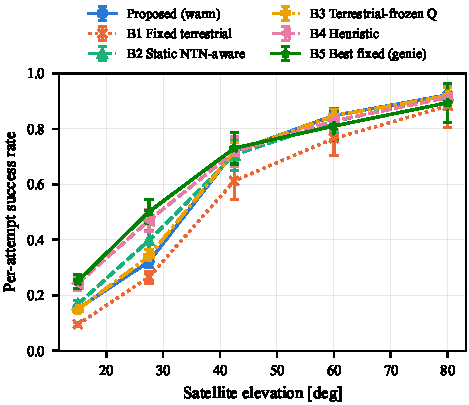
\includegraphics[width=\columnwidth]{fig2_success_vs_elevation.pdf}
\caption{Per-attempt success rate vs.\ elevation (mean, 95\% CI over runs).}
\label{fig:elev}
\end{figure}

\begin{figure}[t]
\centering
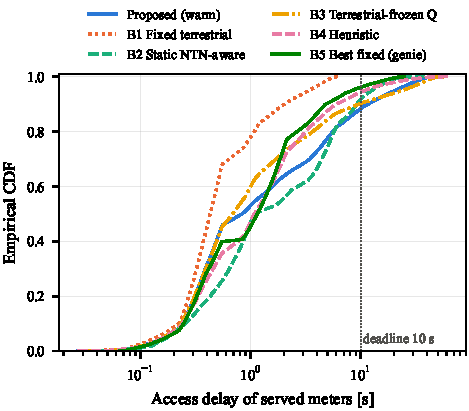
\includegraphics[width=\columnwidth]{fig3_delay_cdf.pdf}
\caption{Access-delay CDF of \emph{served} meters. The dotted line marks the 10-s deadline. B1 serves only 62\% of meters.}
\label{fig:cdf}
\end{figure}

\subsection{Failure Causes and Learned Behaviour}
Fig.~\ref{fig:fail} shows the ground-truth failures and the chosen actions over the pass. Collisions dominate near both horizons, where the alarm burst and backlogged meters crowd the small CE2 pool. Misses are concentrated at low elevation. The proposed controller lowers $p$ during the collision-heavy phases and keeps moderate CE2 repetitions (40--70) throughout. The cause-blind ablation switches to 128 repetitions late in the pass and consumes 11\% more airtime for slightly lower success. Timeouts remain a small share (2.7\% of attempts), as expected for a 10\% stale-GNSS population.

\begin{figure*}[t]
\centering
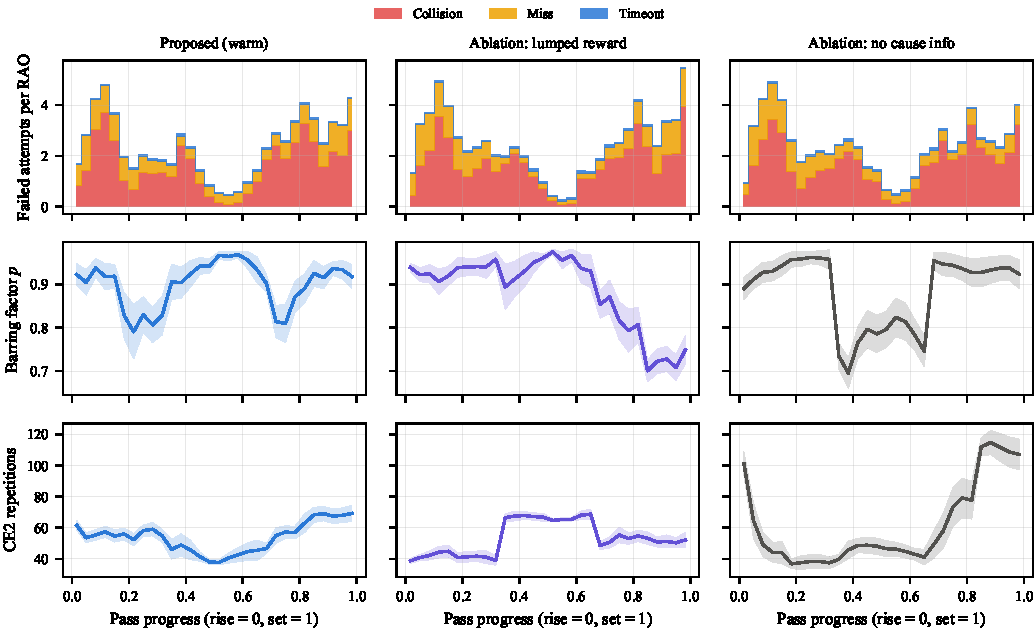
\includegraphics[width=\textwidth]{fig4_failure_breakdown.pdf}
\caption{Ground-truth failure causes (top) and chosen barring factor and CE2 repetitions (mean, 95\% CI) over normalised pass time, for the proposed controller and the two ablations.}
\label{fig:fail}
\end{figure*}

\subsection{Learning within a Pass}
Fig.~\ref{fig:conv} compares warm and cold start. The warm-start reward is higher than the cold-start reward at every phase of the pass. The cold-start learner improves steadily over the first half of the pass but never reaches the warm-start reward. This supports pass-to-pass transfer of the Q-table, rather than learning from scratch within one visibility window. The per-attempt success of both learners stays below that of B5, which uses heavier repetitions.

\begin{figure}[t]
\centering
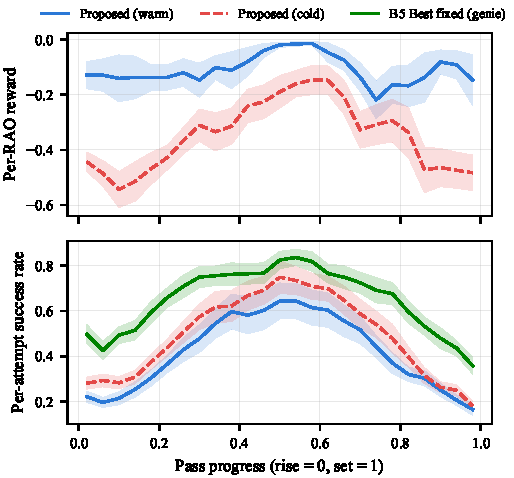
\includegraphics[width=\columnwidth]{fig5_convergence.pdf}
\caption{Per-RAO reward and per-attempt success over the pass: warm vs.\ cold start, with the genie static reference B5.}
\label{fig:conv}
\end{figure}

\subsection{Sensitivity}
Fig.~\ref{fig:sens} reports the gain in $P_s^{\le D}$ over B2 and B5 as a function of load $N$ and coupling loss $\mu_L$ (4 passes $\times$ 4 seeds per cell). B5 keeps the action tuned at the nominal point.
\begin{itemize}
\item \emph{Low and nominal load.} At $N\le1000$, the controller is 8--10~pp below B5 and about 2~pp below B2.
\item \emph{High load.} At $N=3000$ and $5000$, it outperforms B5 by 8.1 and 4.6~pp and the heuristic by 6.5 and 4.4~pp (pooled over $\mu_L$; $p_{\mathrm{Holm}}<0.05$). There, the fixed high-repetition configuration overloads the CE2 pool. For outdoor meters ($\mu_L=0$), its median airtime per served meter grows to 8--15~s, which is 2.8--3.1$\times$ that of the proposed controller.
\end{itemize}

Other sweeps (Proposed / B2 / B4 or B5):
\begin{itemize}
\item \emph{Stale-GNSS share} 0--30\%: 0.69--0.65 / 0.68--0.65 / B5 0.77--0.72.
\item \emph{NPRACH base period} 160--640~ms: 0.69--0.61 / 0.68--0.64 / B4 0.74--0.72.
\item \emph{Synthetic altitudes} 500--800~km: 0.80--0.59 / 0.79--0.58 / B4 0.84--0.66.
\item \emph{GNSS-free detection regime}: all schemes collapse, and the proposed controller is lowest (0.10, vs.\ 0.13--0.17).
\end{itemize}

\begin{figure*}[t]
\centering
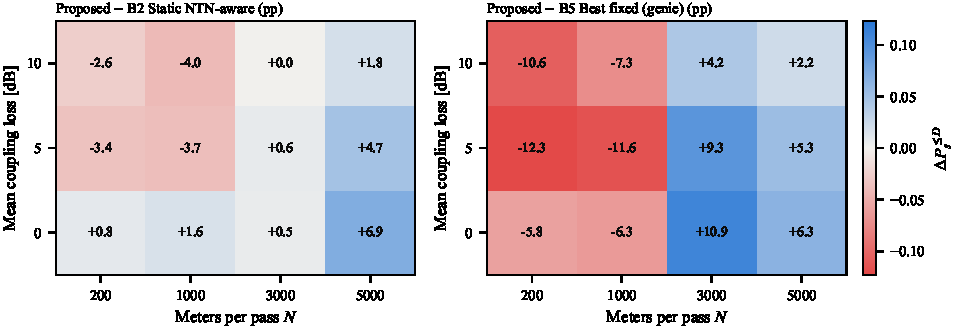
\includegraphics[width=0.85\textwidth]{fig6_sensitivity.pdf}
\caption{Gain of the proposed controller in 10-s access success over B2 (left) and the nominal-tuned genie B5 (right), in percentage points, vs.\ meters per pass and mean coupling loss.}
\label{fig:sens}
\end{figure*}

\subsection{Design Iteration (Disclosure)}
The first, pre-declared design (v1) had no deferral term ($w_d=0$) and only 30 pre-training passes. It reached only $P_s^{\le D}=0.492$, with 11-s mean delay, and its warm start was worse than cold start (0.558). Before rerunning, we declared exactly two changes and their values: the deferral term and the 120-pass pre-training schedule. v1 and v2 are both reproducible from the released configurations, and both are reported in the repository.

\section{Discussion and Limitations}
The controller is an energy-efficient, load-robust alternative to static configuration. It is not a uniform improvement: a genie-tuned fixed setting is better at the load it was tuned for. The proposed controller removes the need for that tuning and degrades more gracefully when the load departs from it. Two of our hypotheses did not hold. The satellite-geometry state features did not help, and the cause-separated weights add only about 1.5~pp over a lumped reward; most of the cause benefit comes through the state.

The limitations of this study are as follows:
\begin{itemize}
\item one ground site and one satellite in view at a time;
\item no capture effect;
\item an assumed detection-curve slope;
\item a stylised timing-error model;
\item B5 tuned on the test passes;
\item a load estimator that is biased at very low load.
\end{itemize}

\section{Conclusion}
We presented an observable, cause-aware tabular Q-learning controller for NB-IoT NTN random access. We evaluated it on real LEO passes under a standards-anchored link and detection model. It matches a static NTN-aware configuration at 9\% lower airtime, no fixed configuration is better on both success and airtime, and it outperforms the nominal-tuned best configuration by up to 8~pp under heavy load. It does not reach the best static configuration at its tuning point. Future work includes multi-satellite visibility, learned repetition thresholds per CE level, and validation on a hardware NTN testbed such as~\cite{kodheli2021ra}.

\section*{Reproducibility}
Code, configuration (v1 and v2), TLEs, seeds and all result files are in the project repository. \texttt{python main.py} regenerates every number and figure in about 50~minutes on four CPU cores.

\bibliographystyle{IEEEtran}
\bibliography{refs}

\end{document}
